\chapter{Results and Evaluation}
\label{sec:evaluation}

In this section, we describe an automated evaluation framework that measures both the **quality of chatbot responses** (via semantic similarity to an expected answer) and the **retrieval effectiveness** of the underlying vector-based search. The code snippet below outlines how queries, expected answers, and reference data are used to generate numerical scores. Additionally, we present the relevant mathematical formulations to clarify how these scores are computed.

\subsection{Mathematical Foundations}
\label{subsec:math-foundations}

\noindent\textbf{Cosine Similarity.}
Let $\mathbf{x}$ and $\mathbf{y}$ be two $d$-dimensional embeddings (vectors) derived from textual inputs (e.g., a \emph{ground-truth} sentence vs.\ a \emph{chatbot} response). We define the cosine similarity as:
\begin{equation}
  \text{cos\_sim}(\mathbf{x}, \mathbf{y}) \;=\; \frac{\mathbf{x} \cdot \mathbf{y}}{\|\mathbf{x}\|\;\|\mathbf{y}\|},
  \label{eq:cosine-sim}
\end{equation}
where $\mathbf{x} \cdot \mathbf{y}$ is the dot product and $\|\mathbf{x}\|$ is the Euclidean norm of $\mathbf{x}$. The result lies in $[-1, 1]$, but for typical sentence embeddings, values are usually in $[0,1]$.

\noindent\textbf{Generation Similarity Score.}
For a given user query $q$ with an \emph{expected} answer $A$, let $R$ denote the chatbot’s \emph{response}. We encode both $A$ and $R$ using the same sentence-transformer embedding function $\Phi(\cdot)$, producing $\Phi(A)$ and $\Phi(R)$. The \emph{generation similarity score} $S_\text{gen}(q)$ is then:
\begin{equation}
  S_\text{gen}(q) \;=\; \text{cos\_sim}\!\Bigl(\Phi(A),\, \Phi(R)\Bigr).
  \label{eq:generation-sim}
\end{equation}
A higher value indicates the chatbot’s generated text is semantically closer to the ground-truth.

\noindent\textbf{Retrieval Similarity Score.}
We also measure how well the system’s retriever (e.g., a vector database) surfaces relevant text chunks. For each query $q$, we fetch the top-$k$ documents $D_1, D_2, \ldots, D_k$ from the retriever. Each document $D_i$ has content that we embed as $\Phi(D_i)$. The \emph{retrieval similarity score} $S_\text{retr}(q)$ is defined as the average similarity of each retrieved chunk to the expected answer embedding $\Phi(A)$:
\begin{equation}
  S_\text{retr}(q) \;=\; \frac{1}{k}\,\sum_{i=1}^{k} \text{cos\_sim}\!\Bigl(\Phi(A),\, \Phi(D_i)\Bigr).
  \label{eq:retrieval-sim}
\end{equation}
If $S_\text{retr}(q)$ is consistently high, it indicates the retriever is pulling documents semantically aligned with the correct answer.

\subsection{Evaluation Code}
\label{subsec:evaluation-code}

\begin{lstlisting}[language=Python, caption={Evaluation Code for Chatbot Responses and Retrieval Quality}, basicstyle=\small\ttfamily]
import os
import time
import logging
import numpy as np
import plotly.graph_objects as go
from sentence_transformers import SentenceTransformer, util

# Import your LLM chain initialization and retrieval functions.
from app import initialize_llm, long_running_task, docsearch, PROMPT

# Set up logging
logging.basicConfig(level=logging.INFO)

# Load a SentenceTransformer model for semantic similarity evaluation.
similarity_model = SentenceTransformer('all-mpnet-base-v2')

def semantic_similarity(expected: str, response: str) -> float:
    """
    Computes the cosine similarity between the expected and response text.
    Returns a float between 0 and 1.
    """
    embedding_expected = similarity_model.encode(expected, convert_to_tensor=True)
    embedding_response = similarity_model.encode(response, convert_to_tensor=True)
    cosine_sim = util.pytorch_cos_sim(embedding_expected, embedding_response)
    return cosine_sim.item()

# Large test dataset based on MedlinePlus diseases.
test_data = [
    {
        "query": "What are the common symptoms of asthma?",
        "expected": "Asthma symptoms include wheezing, shortness of breath, chest tightness, and coughing.",
        "reference": "MedlinePlus. Asthma. https://medlineplus.gov/asthma.html"
    },
    ...
]

def get_chatbot_response(query: str, context: str = "") -> str:
    """
    Runs your QA chain for a given query.
    """
    input_data = {"query": query, "context": context}
    llm = initialize_llm()
    response = long_running_task(input_data, llm)
    return response.strip()

def evaluate_retrieval(query: str, expected: str, k: int = 5) -> float:
    """
    Evaluates retrieval quality by fetching the top k documents for a query
    and computing the average semantic similarity between each document's content
    and the expected answer.
    """
    retriever = docsearch.as_retriever(search_kwargs={'k': k})
    docs = retriever.invoke(query)
    if not docs:
        return 0.0
    scores = [semantic_similarity(expected, doc.page_content) for doc in docs]
    return np.mean(scores)

def evaluate_responses():
    """
    Evaluates chatbot responses against expected answers using semantic similarity,
    and measures retrieval quality.
    Returns lists of similarity scores and retrieval scores.
    """
    similarity_scores = []
    retrieval_scores = []
    
    for test in test_data:
        query = test["query"]
        expected = test["expected"]
        
        # Retrieve chatbot response.
        response = get_chatbot_response(query, context="")
        sim_score = semantic_similarity(expected, response)
        similarity_scores.append(sim_score)
        
        # Evaluate retrieval quality using top-5 documents.
        ret_score = evaluate_retrieval(query, expected, k=5)
        retrieval_scores.append(ret_score)
        
        print(f"Query:                     {query}")
        print(f"Expected Answer:           {expected}")
        print(f"Chatbot Response:          {response}")
        print(f"Semantic Similarity Score (Generation): {sim_score:.2f}")
        print(f"Average Retrieval Similarity Score (top-5): {ret_score:.2f}")
        print("-" * 80)
    
    return similarity_scores, retrieval_scores

def plot_evaluation(similarity_scores, retrieval_scores):
    """
    Uses Plotly to plot the semantic similarity scores for generation and retrieval,
    and saves the graph as a PNG file.
    """
    test_case_indices = list(range(len(test_data)))
    
    fig = go.Figure()
    fig.add_trace(go.Scatter(
        x=test_case_indices,
        y=similarity_scores,
        mode='lines+markers',
        name='Generation Similarity'
    ))
    fig.add_trace(go.Scatter(
        x=test_case_indices,
        y=retrieval_scores,
        mode='lines+markers',
        name='Retrieval Similarity'
    ))
    fig.update_layout(
        title="Semantic Similarity Scores per Test Case",
        xaxis_title="Test Case Index",
        yaxis_title="Similarity Score",
        template="plotly_white"
    )
    fig.show()
    # Save the graph as a PNG file
    fig.write_image("evaluation_graph.png")

if __name__ == "__main__":
    # Evaluate responses and collect scores.
    sim_scores, ret_scores = evaluate_responses()
    
    # Plot evaluation metrics using Plotly.
    plot_evaluation(sim_scores, ret_scores)
\end{lstlisting}

\begin{table}[htbp]
    \centering
    \resizebox{\textwidth}{!}{%
    \begin{tabular}{|p{3.5cm}|p{3.8cm}|p{3.8cm}|c|c|}
    \hline
    \textbf{Query} & \textbf{Chatbot Response} & \textbf{Expected Answer} & \textbf{Semantic Similarity} & \textbf{Avg. Retrieval Similarity} \\ 
    \hline
    What are the common symptoms of asthma? 
    & wheezing, shortness of breath, chest tightness
    & wheezing, shortness of breath, chest tightness, coughing 
    & 0.95 
    & 0.70 \\ 
    \hline
    What is anemia and what causes it? 
    & deficiency of red blood cells or hemoglobin; caused by iron deficiency, vitamin deficiency, chronic disease
    & deficiency of red blood cells or hemoglobin commonly caused by iron deficiency, vitamin deficiencies, chronic disease
    & 0.92 
    & 0.70 \\ 
    \hline
    What are the early signs of Alzheimer's disease? 
    & memory loss, confusion, difficulty performing tasks, language problems
    & memory loss, confusion, difficulty performing familiar tasks 
    & 0.94 
    & 0.65 \\ 
    \hline
    What types of arthritis exist and how are they treated? 
    & osteoarthritis, rheumatoid arthritis; treated with anti-inflammatory drugs, pain relievers, DMARDs, physical therapy
    & osteoarthritis, rheumatoid arthritis; treated with pain relievers, anti-inflammatory drugs, physical therapy 
    & 0.92 
    & 0.64 \\ 
    \hline
    What is atrial fibrillation and what are its risks? 
    & irregular heartbeat; risks include stroke, heart failure, blood clots
    & irregular heartbeat; stroke, heart failure, other heart complications 
    & 0.87 
    & 0.68 \\ 
    \hline
    \end{tabular}}
    \label{tab:evaluation-results}
    \caption{Evaluation Results of Chatbot Responses}
    \end{table}

    \begin{longtable}{|p{3.5cm}|p{9.1cm}|c|}
        \hline
        \textbf{Questions} & \textbf{Chatbot Response} & \textbf{Rate (1-10)} \\ 
        \hline
         i am feeling shortness of breath and my heart is beating fast and chest pain with discomfort what should i do & You should call your provider or dial 911 immediately if you are experiencing these symptoms. These could be signs of a serious medical condition like a heart attack, pulmonary embolism, or angina. It is essential to seek immediate medical attention to prevent further complications and receive prompt treatment. & 7.0 \\ 
        \hline
         i am referred to Cardiac rehabilitation can you help me
        why this is referred from my doctor & You have been referred to cardiac rehabilitation because your healthcare provider believes it will benefit you in managing and improving your heart health after experiencing a heart problem such as a heart attack, coronary artery disease, or heart surgery. Cardiac rehab is designed to help patients recover from these conditions by providing education on heart-healthy lifestyle changes, supervised exercise programs, and emotional support. The goal of cardiac rehab is to reduce the risk of future cardiovascular events and improve overall quality of life. & 7.0 \\ 
        \hline
         What should I do if I have a cardiac arrest &If you suspect someone is experiencing cardiac arrest, call for emergency medical assistance immediately (911 in the US) and begin performing CPR if trained to do so. Cardiopulmonary resuscitation (CPR) can help keep oxygen flowing to the brain and other vital organs until professional help arrives & 7.0 \\ 
        \hline
         i am experiencing lot a chest burning and pain in my stomach what should i do & Chest burning and pain in the stomach can be caused by various reasons. It is recommended that you seek immediate medical attention if you are currently being treated for cancer, unable to pass stool, vomiting blood or have blood in your stool (especially if bright red, maroon or dark, tarry black), experiencing sudden, sharp abdominal pain, have tenderness in the belly or rigidity and hardness of the abdomen.
         & 7.5 \\ 
        \hline
         i am having diarrhea  from past 4 days what should i do to make it stop & Chest burning and pain in the stomach can be caused by various reasons. It is recommended that you seek immediate medical attention if you are currently being treated for cancer, unable to pass stool, vomiting blood or have blood in your stool (especially if bright red, maroon or dark, tarry black), experiencing sudden, sharp abdominal pain, have tenderness in the belly or rigidity and hardness of the abdomen.
         & 7.5 \\ 
        \hline
         i am experiencing lot a chest burning and pain in my stomach what should i do &  Based on the given context, here are some steps you can take to manage your diarrhea:
        
                1. Drink plenty of fluids: Aim for at least 8-10 glasses of clear liquids per day. These should contain salts and simple sugars if you don't have diabetes. If you do, use sugar-free fluids with careful monitoring of blood sugars.
                
                2. Eat small meals: Instead of three large meals, eat smaller meals more frequently throughout the day.
                
                3. Include salty foods: Consume salty foods like pretzels, soup, and sports drinks to replace lost electrolytes. However, check with your doctor if you have kidney disease before increasing your salt intake.
                
                4. Eat high-potassium foods: Bananas, potatoes without the skin, and watered-down fruit juices are good sources of potassium. Check with your doctor if you have kidney disease before increasing your potassium intake.
                
                5. Avoid certain foods: Certain foods may worsen diarrhea, so try to avoid them. These include dairy products, alcohol, caffeine, fatty or fried foods, spicy foods, and citrus fruits.
                
                6. Be aware of medication interactions: If you're taking any medications, be sure to consult your doctor before stopping or adjusting their dosage.
                
                7. Contact your healthcare provider: If your diarrhea persists for more than a few days or if it is accompanied by other symptoms such as bleeding from the rectum, nausea, vomiting, or constipation, contact your doctor immediately.
                & 8 \\ 
        \hline
         i have this body itching from two days what would be the issue &   If you are experiencing a persistent cough or sneezing, it is best to consult a healthcare provider for proper diagnosis and treatment. In the meantime, you can try the following home remedies to provide some relief:
        
                1. Drink plenty of fluids: Staying hydrated can help thin out mucus and make it easier to clear your airways.
                
                2. Gargle with warm salt water: This can help soothe a sore throat and reduce inflammation.
                
                3. Use a humidifier: Adding moisture to the air can help relieve congestion and coughing.
                
                4. Take over-the-counter medications as needed: Non-drowsy antihistamines like Claritin or Zyrtec may provide relief from allergy symptoms, while decongestants like Sudafed can help clear nasal congestion.
                
                5. Avoid triggers: If you know what is causing your allergies (such as pollen or pet dander), try to avoid exposure to these triggers.
                
                6. Get enough rest: Allowing your body to rest and recover can help speed up the healing process.
                
                7. Monitor symptoms: If symptoms persist or worsen, seek medical attention immediately.
                & 8 \\ 
        \hline
         i am sneezing continuously nonstop from past one hour how to control it &  It is difficult to determine the exact cause of your body itching without a physical examination and medical history by a healthcare provider. However, based on the information you've provided, it could be due to a variety of reasons such as allergic reactions, skin irritation, infections or even underlying medical conditions like eczema or psoriasis. It is recommended that you consult with a doctor for proper diagnosis and treatment.
                & 8 \\ 
        \hline
        \caption{Human Centric Evaluation}
        \label{tab:Human Centric Evaluation}
        \end{longtable}
        
    
    

\subsection{Workflow and Interpretation}
\begin{enumerate}
    \item \textbf{Load Test Cases.} Each entry in \texttt{test\_data} contains:
    \begin{itemize}
        \item \texttt{query}: The user’s question.
        \item \texttt{expected}: A short, correct answer from medical references.
        \item \texttt{reference}: A citation URL.
    \end{itemize}
    \item \textbf{Generation Similarity.}  
    The system obtains the chatbot’s free-form answer and compares it to the ground-truth (\texttt{expected}) using Equation~\ref{eq:generation-sim}. 
    \begin{equation}
      S_\mathrm{gen} = \text{cos\_sim}\!\Bigl(\Phi(\text{expected}), \,\Phi(\text{response})\Bigr).
      \label{eq:generation-sim}
    \end{equation}
    A higher $S_\mathrm{gen}$ indicates the chatbot’s answer is semantically close to the reference.

    \item \textbf{Retrieval Similarity.}  
    Independently, the code checks the top-$k$ retrieved documents to see how aligned they are with the expected text (Equation~\ref{eq:retrieval-sim}):
    \begin{equation}
      S_\mathrm{retr} = \frac{1}{k} \sum_{i=1}^k \text{cos\_sim}\!\Bigl(\Phi(\text{expected}), \,\Phi(D_i)\Bigr),
      \label{eq:retrieval-sim}
    \end{equation}
    where $D_i$ is the $i$-th retrieved document chunk. A higher $S_\mathrm{retr}$ suggests the vector store is returning relevant context.
\end{enumerate}

\subsection{Significance in the Thesis}
\begin{itemize}
    \item \textbf{Quantitative Insight.} By assigning numerical scores to both the final answer (generation) and the retrieved documents, the methodology pinpoints whether errors stem from the \emph{retrieval} stage or the \emph{generation} stage.
    \item \textbf{Scalability.} New questions can be added to \texttt{test\_data} without retraining the entire model, allowing continuous monitoring of the system’s performance.
    \item \textbf{Guidance for Improvement.} 
    \begin{itemize}
        \item If retrieval scores ($S_\mathrm{retr}$) are consistently high but generation scores ($S_\mathrm{gen}$) are low, the problem may lie in the LLM’s prompt or response generation logic.
        \item If retrieval scores are low, the embedding or vector store configuration might need refinement.
    \end{itemize}
\end{itemize}

\noindent
Overall, this evaluation approach, supported by Equations~\ref{eq:cosine-sim}, \ref{eq:generation-sim}, and \ref{eq:retrieval-sim}, provides a rigorous, automated way to measure how effectively the chatbot answers medical queries and how well its retrieval subsystem surfaces relevant evidence from the knowledge base.

\label{sec:results}

\section{Introduction to Chatbot Interactions}
This section presents selected screenshots that illustrate how our chatbot addresses the research questions posed in this thesis. Each figure demonstrates different functionalities, user roles, and response flows, highlighting how the system handles both student and patient interactions.

\section{Booking an Appointment (Patient Perspective)}
\label{sec:booking-appointment}

\begin{figure}[htbp]
    \centering
    % Adjust the width or use scale if necessary
    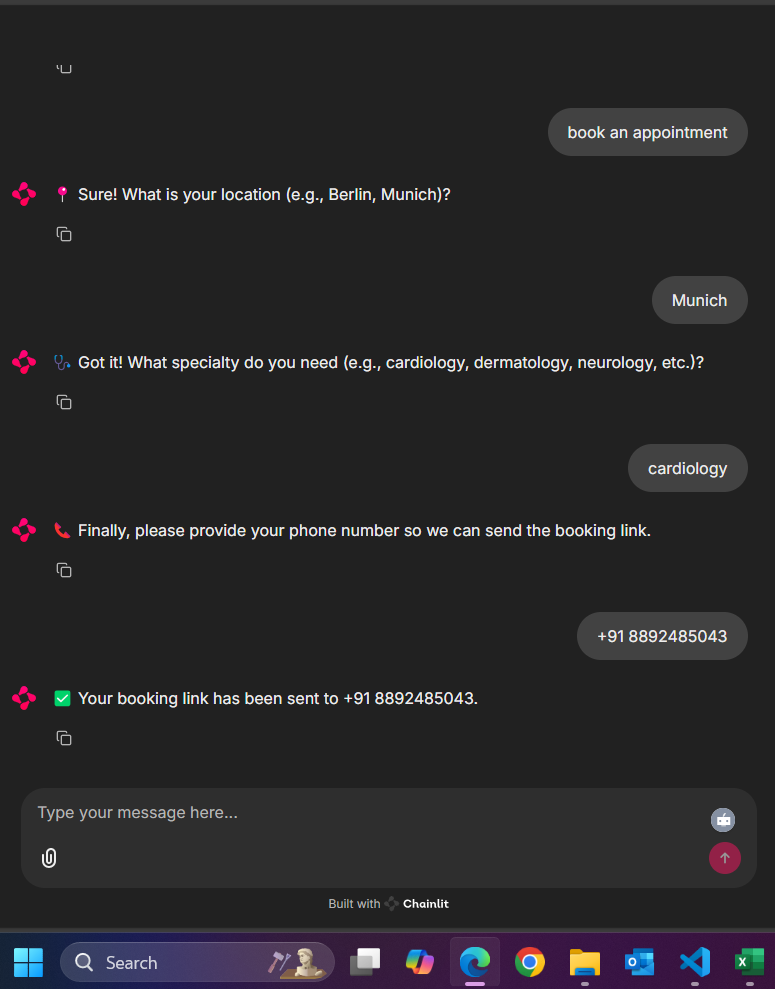
\includegraphics[width=0.85\textwidth]{Images/doclink1.png}
    \caption{A patient booking an appointment. The chatbot requests the location (e.g., Munich) and the specialty (e.g., Cardiology), then collects the user’s phone number to send a booking link.}
    \label{fig:book-appointment}
\end{figure}

As shown in Figure~\ref{fig:book-appointment}, the chatbot confirms the patient’s location and medical specialty. Once the user provides a phone number, the system sends a direct link for appointment scheduling, thereby streamlining the booking process.

\section{Student Role: Medical Explanations}
\label{sec:student-role}


\begin{figure}[htbp]
    \centering
    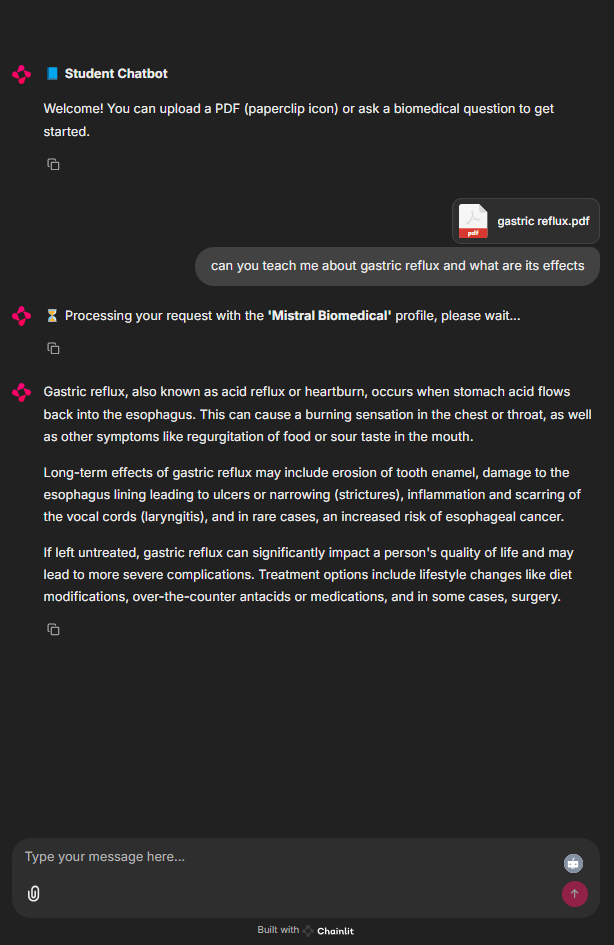
\includegraphics[width=0.85\textwidth]{Images/pdfquestion.png}
    \caption{A student asking for detailed medical information. The chatbot provides an academic explanation suited for learning, referencing embedded content.}
    \label{fig:student-chatbot}
\end{figure}

Figure~\ref{fig:student-chatbot} highlights how a user with the \emph{Student} role can request deeper, evidence-based information. The chatbot uses context from embedded academic texts, ensuring that explanations remain precise and pedagogically useful.

\section{Symptom Analysis and Guidance}
\label{sec:patient-symptoms}

\begin{figure}[htbp]
    \centering
    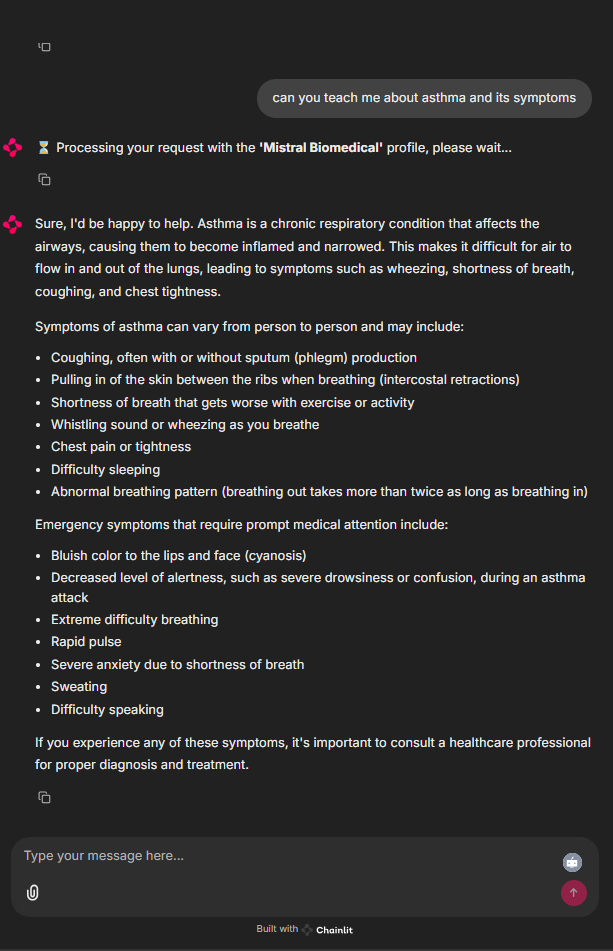
\includegraphics[width=0.85\textwidth]{Images/stuentquestion.png}
    \caption{A student asking specific medical questions (e.g., asthma-related issues) in order to learn more. The chatbot responds with context-aware guidance, referencing standard medical guidelines and educational sources.}
    \label{fig:patient-symptoms}
\end{figure}

In Figure~\ref{fig:patient-symptoms}, a patient reports respiratory symptoms. The chatbot, using retrieval-augmented generation (RAG), provides relevant medical guidance while filtering out any sensitive data at the edge to maintain privacy compliance.

\section{Managing Gastrointestinal Issues}
\label{sec:diarrhea-question}

\begin{figure}[htbp]
    \centering
    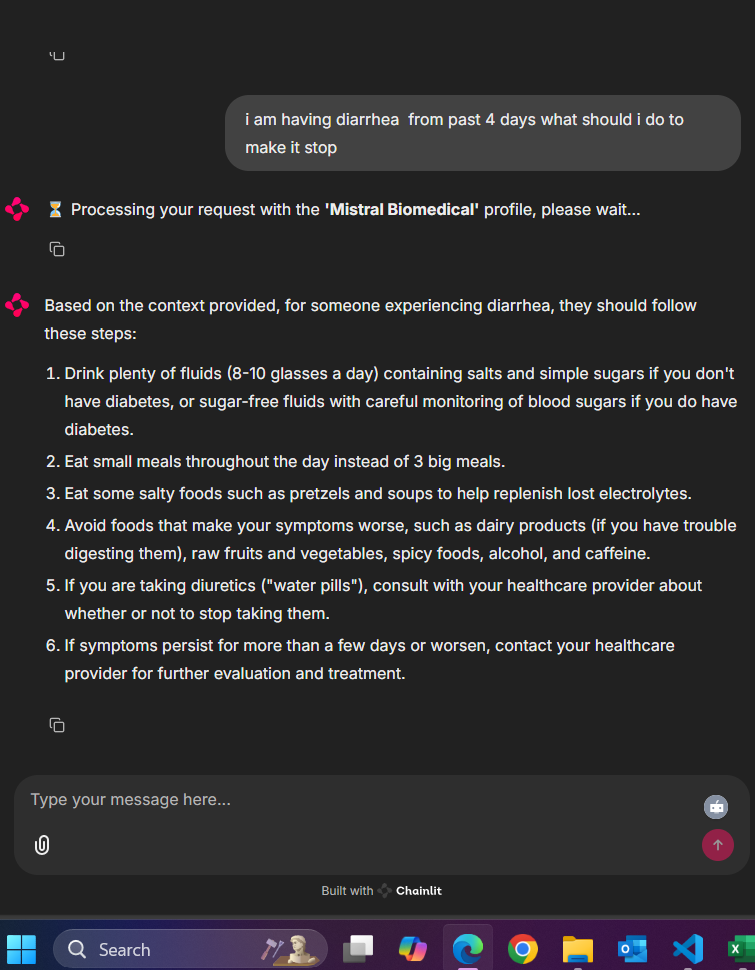
\includegraphics[width=0.85\textwidth]{Images/patientsymptoms.png}
    \caption{A patient scenario discussing diarrhea symptoms for four days. The chatbot suggests dietary measures and advises contacting a healthcare professional if symptoms worsen.}
    \label{fig:diarrhea-question}
\end{figure}

Figure~\ref{fig:diarrhea-question} demonstrates how the chatbot uses user inputs (e.g., “four days of diarrhea”) to provide context-appropriate advice, such as recommending fluid intake and dietary modifications. The system also cautions the user to consult a professional if conditions do not improve.

\section{Provider Recommendations}
\label{sec:doctor-recommendations}

\begin{figure}[htbp]
    \centering
    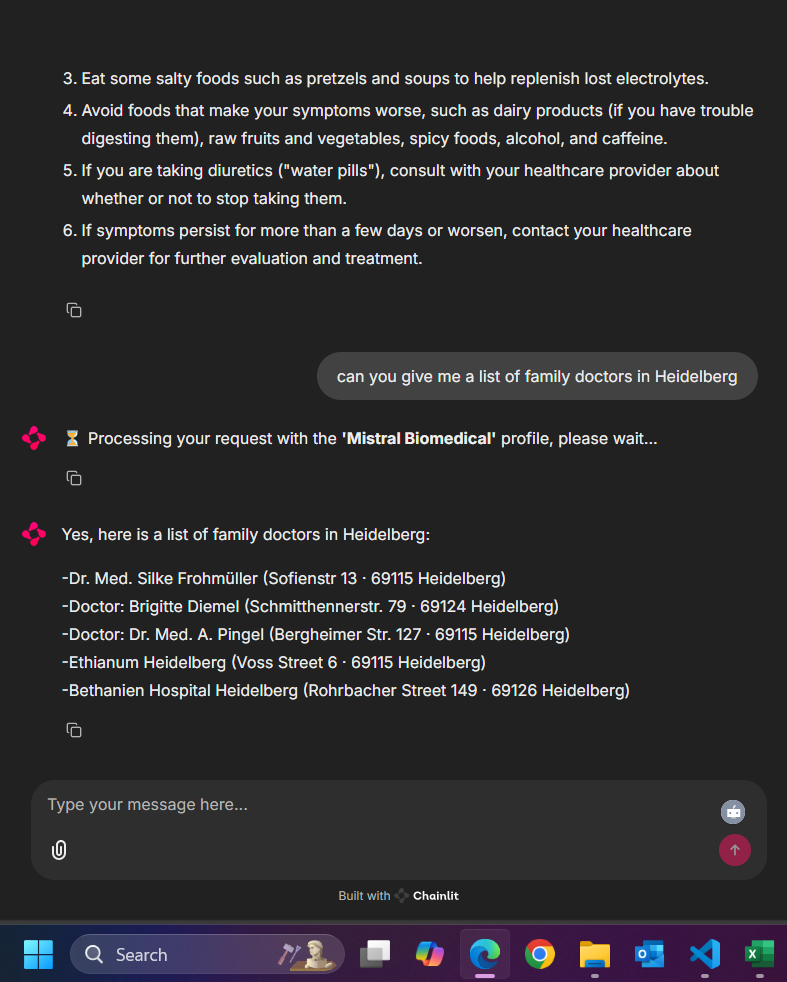
\includegraphics[width=0.85\textwidth]{Images/doctorrecom.png}
    \caption{Chatbot suggesting a list of nearby family doctors in Heidelberg, filtered by location and specialty.}
    \label{fig:doctor-recom}
\end{figure}
In Figure~\ref{fig:doctor-recom}, the chatbot generates a list of nearby healthcare providers based on the patient’s location. This feature demonstrates the system’s ability to integrate location-based data with a specialty filter, simplifying the referral process.


\section{Agentic Booking System}

\begin{figure}[H]
  \centering
  
\includegraphics[width=0.3\textwidth]{Images/appointmentlink.png}
  \caption{Agentic AI demonstration: The system automatically integrates with Twilio 
    to send the user an appointment booking link for a cardiology specialist in Munich.}
  \label{fig:agentic_ai_booking}
\end{figure}

\section{Discussion of Chatbot Interaction Results}
Overall, these screenshots illustrate the chatbot’s capacity to:
\begin{itemize}
    \item \textbf{Identify user roles} (patient vs.\ student) and deliver tailored content.
    \item \textbf{Provide medical insights} based on retrieval-augmented generation (RAG).
    \item \textbf{Offer practical guidance} such as appointment booking and provider recommendations.
\end{itemize}

These functionalities address the research questions outlined in the earlier chapters, showcasing how the system can effectively serve both educational and clinical needs in a unified platform.

